\documentclass{Z}

%%\VignetteIndexEntry{party with the mob}
%%\VignetteDepends{mlbench,colorspace}

%% packages
\usepackage{amsmath}

%% neet no \usepackage{Sweave}


%% commands
\newcommand{\ui}{\underline{i}}
\newcommand{\oi}{\overline{\imath}}
\newcommand{\argmin}{\operatorname{argmin}\displaylimits}

%% author/title
\author{Achim Zeileis\\Wirtschaftsuniversit\"at Wien \And
        Torsten Hothorn\\Friedrich-Alexander-Universit\"at\\Erlangen-N\"urnberg \And
	Kurt Hornik\\Wirtschaftsuniversit\"at Wien}
\Plainauthor{Achim Zeileis, Torsten Hothorn, Kurt Hornik}

\title{\pkg{party} with the \code{mob}: Model-based Recursive Partitioning in \proglang{R}}
\Plaintitle{party with the mob: Model-based Recursive Partitioning in R}
\Shorttitle{\pkg{party} with the \texttt{mob}}

\Keywords{parametric models, object-orientation, recursive partitioning}

%% abstract
\Abstract{
  The \pkg{party} package \citep{Hothorn+Hornik+Zeileis:2006a} provides
  the function \code{mob()} implementing a recently suggested algorithm
  for \underline{mo}del-\underline{b}ased recursive partitioning
  \citep{Zeileis+Hothorn+Hornik:2005}. The basic steps are: (1)~fit a
  parametric model to a data set, (2)~test for parameter instability over
  a set of partitioning variables, (3)~if there is some overall parameter
  instability, split the model with respect to the variable associated with
  the highest instability, (4)~repeat the procedure in each of the child nodes.
  It is discussed how these steps of the conceptual algorithm are translated
  into computational tools in an object-oriented manner, allowing the user to
  plug in various types of parametric models. The outcome is a tree where
  each node is associated with a fitted parametric model that can be
  effectively visualized and summarized.
}

\begin{document}


\section{Motivation}
\label{sec:motivation}

Consider a parametric model $\mathcal{M}(Y, \theta)$
with (possibly vector-valued) observations $Y$ and a
$k$-dimensional vector of parameters $\theta$. This model 
could be a (possibly multivariate) normal distribution for $Y$, or some
kind of regression model when $Y = (y, x)$ can be split up into a dependent variable
$y$ and regressors $x$. An example for the latter could be a linear regression
model $y = x^\top \theta$ or a generalized linear model (GLM) or a survival 
regression.

Given $n$ observations $Y_i$ ($i = 1, \dots, n$) the model can be fitted
by minimizing some objective function $\Psi(Y, \theta)$, e.g., a residual sum of squares
or a negative log-likelihood leading to ordinary least squares (OLS) or maximum
likelihood (ML) estimation.

If a global model for all $n$ observations does not fit well and further
covariates $Z_1, \dots, Z_\ell$ are available, it might be possible to partition
the $n$ observations with respect to these variables and find a fitting model
in each cell of the partition. The algorithm described here tries to find
such a partition adaptively using a greedy forward search. This procedure is
implemented in the function \code{mob()} and described in more detail in the following
section. However, we we will state some goals and design principles in advance.

To translate the model-based partitioning problem into \proglang{R}, we start with
a formula description of the variables involved. This formula should be of type
\verb:y ~ x1 + ... + xk | z1 + ... + zl: where the variables on the
left of the \code{|} specify the data $Y$ and the variables on the right specify the
partitioning variables $Z_j$. Classical regression trees usually have a univariate
response $Y$ and various partitioning variables, i.e., could be specified as
\verb:y ~ 1 | z1 + ... + zl:. Structural change models, on the other hand, are usually
regression models that are segmented with respect to a single partitioning variable,
typically time: \verb:y ~ x1 + ... + xk | z:.

The type of models $\mathcal{M}$ to be used with \code{mob()} should not be
confined (by the implementation), hence we have written an object-oriented 
implementation. The idea is that $\mathcal{M}$ is translated into software
by a model of class ``\code{StatModel}'' as provided by the \pkg{modeltools}
package. The algorithm the relies on various methods being available for these
models. The ``\code{StatModel}'' objects \code{linearModel} and \code{glinearModel},
implementing (generalized) linear regression models, are readily available in
\pkg{modeltools}, others can easily be user-defined.


\section{The model-based recursive partitioning algorithm}
\label{sec:algorithm}

The basic idea is to grow a tee in which every node is associated with a model
of type $\mathcal{M}$. To assess whether splitting of the node is necessary a
fluctuation test for parameter instability is performed. If there is significant instability
with respect to any of the partitioning variables $Z_j$, the node is splitted
into $B$ locally optimal segments (currently only $B = 2$ is implemented)
and then the procedure is repeated in each of the $B$ children.
If no more significant instabilities can be found, the recursion stops.
More precisely, the steps of the algorithm are

\begin{enumerate}
\item Fit the model once to all observations in the current node.
\item Assess whether the parameter estimates are stable with respect to
  every partitioning variable $Z_1, \dots, Z_\ell$. If there is some overall instability,
  select the variable $Z_j$ associated with the highest parameter instability, otherwise
  stop.
\item Compute the split point(s) that locally optimize the objective function $\Psi$.
\item Split the node into child nodes and repeat the procedure.
\end{enumerate}

The details for steps 1--3 are specified in the following.


\subsection{Parameter estimation}

This step of the algorithm is common practice, the only additional 
requirement is (as previously noted) that model has to be of the class
``\code{StatModel}'' as provided by \pkg{modeltools}. Looking at the source
code for the \code{linearModel} provided by this package illustrates how
a simple wrapper to existing \proglang{R} functionality can be written.
In particular, a method to the generic function \code{reweight()} has to
be available. The reason is that it is inefficient to fit a brand-new model
\code{modelobj} (including formula-parsing) in every node---much computation time
is saved if simply \code{reweight(modelobj, weights)} is called in each of the
child nodes. The \code{weights} argument controls which observations go into which
of the child nodes.


\subsection{Testing for parameter instability}

The task in this step of the algorithm is to find out whether the parameters
of the fitted model are stable over each particular ordering implied by
the partitioning variables $Z_j$ or whether splitting the sample with respect
to one of the $Z_j$ might capture instabilities in the parameters and thus improve the fit.
The tests used in this step belong to the class of generalized M-fluctuation
tests \citep{ZeileisHornik2003,Zeileis2005}. For numerical partitioning variables
$Z_j$ the $\sup LM$~statistic is used which is the maximum over all single split
$LM$ statistics. For categorical partitioning variables, a $\chi^2$~statistic is
employed which captures the fluctuation within each of the categories of $Z_j$.

For computing the test statistics and corresponding $p$~values $p_j$ for 
each of the partitioning variables $Z_j$ in \proglang{R}, the only requirement
is that there are methods for the extractor functions \code{estfun()} and 
\code{weights()}. The \code{estfun()} method extracts the empirical estimating
functions (model scores) from the fitted \code{modelobj}, these are the 
main ingredient for M-fluctuation tests. The \code{weights()} method is used
to determine which observations are in the current node (i.e., have a weight
greater than zero) and which are not (i.e., have zero weight).

To determine whether there is some overall instability, it is checked whether
the minial $p$~value $p_{j^*} = \min_{j = 1, \dots, \ell} p_j$ falls below a
pre-specified significance level $\alpha$ (by default $\alpha = 0.05$) or not.
To adjust for multiple testing, the $p$ values can be Bonferroni adjusted
(which is the default). If there is significant instability, the variable $Z_{j^*}$
associated with the minimal $p$~value is used for splitting the node.

\subsection{Splitting}

In this step, the observation in the current node are split with respect
to the chosen partitioning variable $Z_{j^*}$ into $B$ child nodes. Currently,
the infrastructure in \pkg{party} only supports binary splits, i.e., $B = 2$.
For deterimining the split point, an exhaustive search procedure is adopted:
For each conceivable split point, the $B$ child node models are fit and the split
associated with the minimal value of the objective function $\Psi$ is chosen.

Computationally, this means that the fitted model \code{modelobj} is \code{reweight()}ed
for each of the child nodes. The observations entering a child node keep their
current weight while those observations that go into different child nodes receive
zero weight. To compare the objective function $\Psi$, an extractor function
is required to compute it from the fitted \code{modelobj}. This extractor function
can be user-specified and set in \verb:mob_control():, it defaults to \code{deviance()}.


This concludes one iteration of the recursive partitioning algorithm and steps~1--3
are carried out again in each of the $B$ daughter nodes until no significant 
instability is detected in step~2.

\section{Illustrations}
\label{sec:illustration}

\subsection{Boston housing data}

Since the analysis by \cite{BreimanFriedman1985}, the Boston housing data are 
a popular and well-investigated empirical basis for illustrating non-linear 
regression methods both in machine learning and statistics
\citep[see][for two recent examples]{Gama2004,Samarovetal2005} and we follow 
these examples by segmenting a bivariate linear regression model for the house
values.

Thus, the model $\mathcal{M}$ used is \code{linearModel} from the \pkg{modeltools}
package which is automatically loaded together with \pkg{party}.

\begin{Schunk}
\begin{Sinput}
> library("party")
\end{Sinput}
\end{Schunk}

The data set is available in package \pkg{mlbench} via

\begin{Schunk}
\begin{Sinput}
> data("BostonHousing", package = "mlbench")
\end{Sinput}
\end{Schunk}

and provides $n = 506$ observations of the median value of owner-occupied
homes in Boston (in USD~1000) along with $14$ covariates including in particular
the number of rooms per dwelling (\code{rm}) and the percentage
of lower status of the population (\code{lstat}). A segment-wise linear relationship between
the value and these two variables is very intuitive, whereas the shape of the influence
of the remaining covariates is rather unclear and hence should be learned from the data.
Therefore, a linear regression model for median value explained by \verb:rm^2:
and \verb:log(lstat): with $k = 3$ regression coefficients is employed and
partitioned with respect to all $\ell = 11$ remaining variables. To facilitate subsequent
commands, the transformations are explicitely stored in \code{BostonHousing}:

\begin{Schunk}
\begin{Sinput}
> BostonHousing$lstat <- log(BostonHousing$lstat)
> BostonHousing$rm <- BostonHousing$rm^2
\end{Sinput}
\end{Schunk}

Choosing appropriate
transformations of the dependent variable and the regressors that enter the linear
regression model is important to obtain a well-fitting model in each segment and
we follow in our choice the recommendations of \cite{BreimanFriedman1985}. Monotonous
transformations of the partitioning variables do not affect the recursive partitioning
algorithm and hence do not have to be performed. However, it is important to distinguish
between numerical and categorical variables for choosing an appropriate parameter 
stability test. The variable \code{chas} is a dummy indicator variable (for tract bounds
with Charles river) and should thus be turned into a factor. Furthermore, the variable
\code{rad} is an index of accessibility to radial highways and takes only 9 distinct
values. Thus it is most appropriately treated as an ordered factor.

\begin{Schunk}
\begin{Sinput}
> BostonHousing$chas <- factor(BostonHousing$chas, levels = 0:1, labels = c("no", "yes"))
> BostonHousing$rad <- factor(BostonHousing$rad, ordered = TRUE)
\end{Sinput}
\end{Schunk}

Both transformations only affect the parameter stability test chosen (step~2), not the splitting
procedure (step~3).

The model is estimated
by OLS, the instability is assessed using a Bonferroni-corrected
significance level of $\alpha = 0.05$ and the nodes are split with a required minimal
segment size of $40$ observations. The control parameters are thus set to

\begin{Schunk}
\begin{Sinput}
> ctrl <- mob_control(alpha = 0.05, bonferroni = TRUE, minsplit = 40,
+   objfun = deviance, verbose = TRUE)
\end{Sinput}
\end{Schunk}

Actually, all of these settings are the defaults except \code{minsplit = 40} and
\code{verbose = TRUE} which causes some information about the fitting process
being written to the screen. The objective function \code{deviance()} extracts in
this case the residual sum of squares from a fitted \code{linearModel} object.

Having collected all building blocks, we can now call the function \code{mob()}
that takes the model specification of the linear regression model \verb:medv ~ lstat + rm:
plus all partitioning variables, along with the \code{data} set, the \code{control}
settings and the \code{model} to be used.

\begin{Schunk}
\begin{Sinput}
> fmBH <- mob(medv ~ lstat + rm | zn + indus + chas + nox + age + dis + rad + tax + crim + b + ptratio,
+   data = BostonHousing, control = ctrl, model = linearModel)
\end{Sinput}
\begin{Soutput}
-------------------------------------------
Fluctuation tests of splitting variables:
                    zn        indus         chas          nox          age
statistic 3.363356e+01 6.532322e+01 2.275635e+01 8.136281e+01 3.675850e+01
p.value   1.176113e-04 1.603635e-11 4.993053e-04 4.138241e-15 2.608438e-05
                   dis          rad          tax         crim            b
statistic 6.903150e+01 1.153641e+02 9.068440e+01 8.655065e+01 3.627629e+01
p.value   2.397851e-12 7.087680e-13 3.257864e-17 2.801011e-16 3.294641e-05
               ptratio
statistic 7.221524e+01
p.value   4.666898e-13

Best splitting variable: tax
Perform split? yes
-------------------------------------------

Node properties:
tax <= 432; criterion = 1, statistic = 115.364

-------------------------------------------
Fluctuation tests of splitting variables:
                    zn       indus      chas          nox        age
statistic 27.785009791 21.33293464 8.0272421 23.774323202 11.9204284
p.value    0.001494064  0.02851930 0.4005192  0.009518732  0.7666366
                   dis          rad          tax         crim         b
statistic 24.268011081 50.481593270 3.523250e+01 3.276813e+01 9.0363245
p.value    0.007601532  0.003437763 4.275527e-05 1.404487e-04 0.9871502
               ptratio
statistic 4.510680e+01
p.value   3.309747e-07

Best splitting variable: ptratio
Perform split? yes
-------------------------------------------

Node properties:
ptratio <= 15.2; criterion = 1, statistic = 50.482

-------------------------------------------
Fluctuation tests of splitting variables:
                    zn       indus        chas         nox         age
statistic 3.233350e+01 22.26864036 12.93407112 22.10510234 20.41295354
p.value   1.229678e-04  0.01504788  0.05259509  0.01622098  0.03499731
                 dis          rad          tax        crim         b
statistic 17.7204735 5.526565e+01 2.879128e+01 20.28503194 6.5549665
p.value    0.1091769 7.112214e-04 6.916307e-04  0.03706934 0.9999522
               ptratio
statistic 4.789850e+01
p.value   4.738855e-08

Best splitting variable: ptratio
Perform split? yes
-------------------------------------------

Node properties:
ptratio <= 19.6; criterion = 1, statistic = 55.266

-------------------------------------------
Fluctuation tests of splitting variables:
                 zn      indus      chas        nox       age        dis
statistic 14.971474 14.6477733 7.1172962 14.3455158 8.2176363 16.1112185
p.value    0.280361  0.3134649 0.5405005  0.3467974 0.9906672  0.1847818
                  rad          tax     crim         b    ptratio
statistic 43.17824350 3.447271e+01 9.340075 8.7773142 10.8469969
p.value    0.03281124 4.281939e-05 0.952996 0.9772696  0.8202694

Best splitting variable: tax
Perform split? yes
-------------------------------------------

Node properties:
tax <= 265; criterion = 1, statistic = 43.178

-------------------------------------------
Fluctuation tests of splitting variables:
                 zn     indus     chas      nox        age       dis        rad
statistic 11.998039 7.3971233 7.227770 9.293619 14.3023962 8.9239826 33.1746444
p.value    0.574642 0.9931875 0.522447 0.911962  0.2886603 0.9389895  0.3926249
                 tax       crim         b    ptratio
statistic 16.6666129 11.7143758 9.9050903 11.5927528
p.value    0.1206412  0.6153455 0.8539893  0.6328381

Best splitting variable: tax
Perform split? no
-------------------------------------------

-------------------------------------------
Fluctuation tests of splitting variables:
                  zn     indus         chas         nox       age        dis
statistic 10.9187926 9.0917078 2.754081e+01 17.39203006 4.6282349 11.9581600
p.value    0.7091039 0.9172303 4.987667e-05  0.08922543 0.9999992  0.5607267
                rad        tax     crim        b   ptratio
statistic 0.2557803 10.9076165 3.711175 3.158329 9.8865054
p.value   1.0000000  0.7106612 1.000000 1.000000 0.8410064

Best splitting variable: chas
Perform split? yes
-------------------------------------------

Splitting factor variable, objective function: 
 no 
Inf 

No admissable split found in ‘chas’
\end{Soutput}
\end{Schunk}

The result is the fitted model \code{fmBH} of class ``\code{mob}'' that contains
the tree with a fitted linear regression associated with every node. Printing
this object will show the splits, their $p$ values and call the \code{print()} method
for the model in each terminal node (i.e., this simply relies on a \code{print()}
method being available for the fitted model and re-uses it).

\begin{Schunk}
\begin{Sinput}
> fmBH
\end{Sinput}
\begin{Soutput}
1) tax <= 432; criterion = 1, statistic = 115.364
  2) ptratio <= 15.2; criterion = 1, statistic = 50.482
    3)*  weights = 72 
Terminal node model
Linear model with coefficients:
(Intercept)        lstat           rm  
     9.2349      -4.9391       0.6859  

  2) ptratio > 15.2
    4) ptratio <= 19.6; criterion = 1, statistic = 55.266
      5) tax <= 265; criterion = 1, statistic = 43.178
        6)*  weights = 63 
Terminal node model
Linear model with coefficients:
(Intercept)        lstat           rm  
     3.9637      -2.7663       0.6881  

      5) tax > 265
        7)*  weights = 162 
Terminal node model
Linear model with coefficients:
(Intercept)        lstat           rm  
    -1.7984      -0.2677       0.6539  

    4) ptratio > 19.6
      8)*  weights = 56 
Terminal node model
Linear model with coefficients:
(Intercept)        lstat           rm  
    17.5865      -4.6190       0.3387  

1) tax > 432
  9)*  weights = 153 
Terminal node model
Linear model with coefficients:
(Intercept)        lstat           rm  
    68.2971     -16.3540      -0.1478  
\end{Soutput}
\end{Schunk}

Looking at the printed output is typically rather tedious, a visualization via
the \code{plot()} method

\begin{Schunk}
\begin{Sinput}
> plot(fmBH)
\end{Sinput}
\end{Schunk}

is much easier to interpret. By default, this produces partial scatter plots of the
variable $y$ against each of the regressors $x_i$ in the terminal nodes. Each scatter
plot also shows the fitted values, i.e., a project of the fitted hyperplane.

\setkeys{Gin}{width=\textwidth}
\begin{figure}[p]
\begin{center}
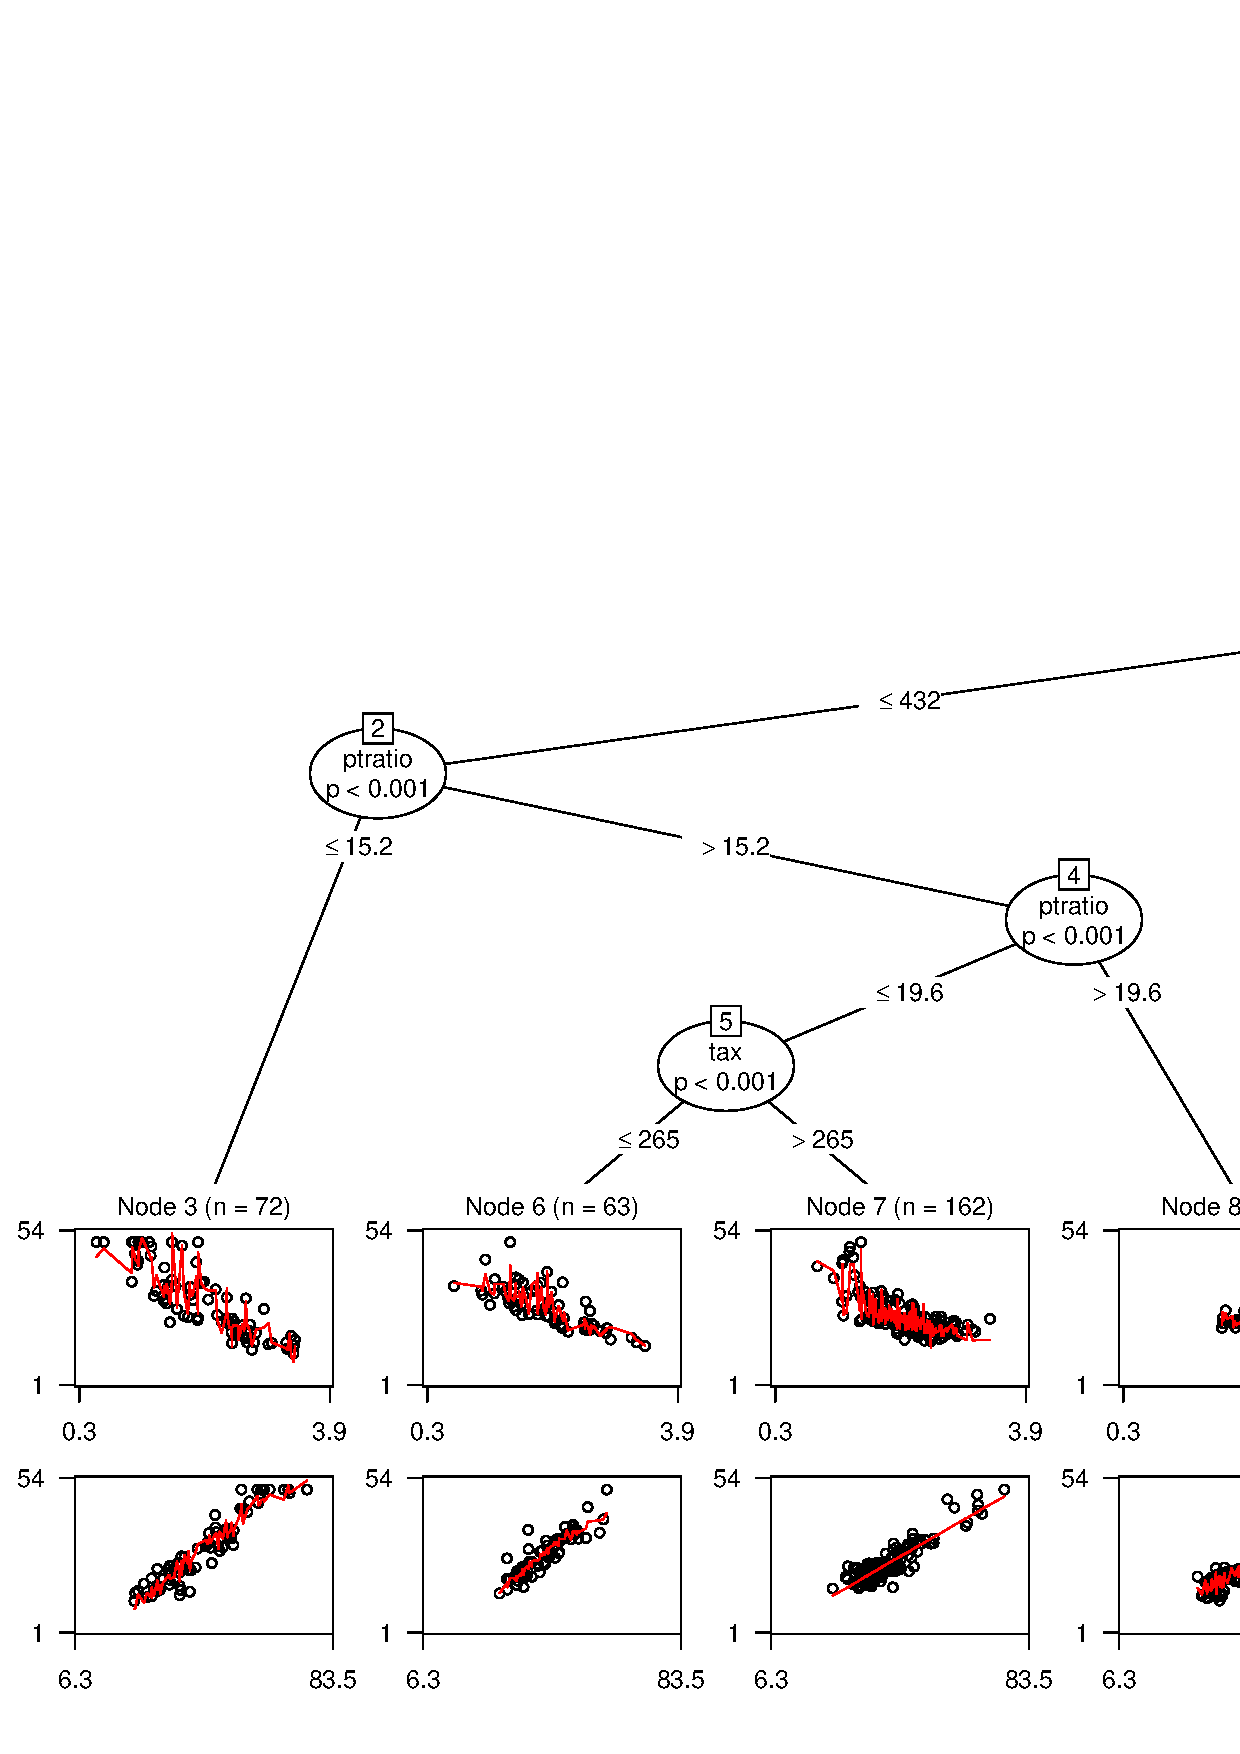
\includegraphics[width=18cm,keepaspectratio,angle=90]{MOB-BostonHousing-plot}
\caption{\label{fig:BostonHousing} Linear-regression-based tree for the Boston housing data.
The plots in the leaves give partial scatter plots for \code{rm} (upper panel) and 
\code{lstat} (lower panel).}
\end{center}
\end{figure}

From this visualization, it can be seen that in the nodes~4, 6, 7 and 8 the increase of
value with the number of rooms dominates the picture (upper panel) whereas in node~9 the
decrease with the lower status population percentage (lower panel) is more pronounced. 
Splits are performed in the variables \code{tax} (poperty-tax rate) and
\code{ptratio} (pupil-teacher ratio).

Various quantities of interest can be computed, provided that the \code{model} used
provides the corresponding methods, e.g., \code{predict()}, \code{residuals()}, \code{logLik()},
\code{coef()} and \code{summary()}. The latter two by default try to extract information
for the terminal nodes, but a \code{node} argument can be set to the node IDs of interest.
As an example, the regression coefficients for the terminal node models can be easily 
extracted by

\begin{Schunk}
\begin{Sinput}
> coef(fmBH)
\end{Sinput}
\begin{Soutput}
  (Intercept)      lstat         rm
3    9.234880  -4.939096  0.6859136
6    3.963720  -2.766287  0.6881287
7   -1.798387  -0.267707  0.6538864
8   17.586490  -4.618975  0.3386744
9   68.297087 -16.354006 -0.1477939
\end{Soutput}
\end{Schunk}

reflecting the differences of the models that can also be seen in the the associated
\code{plot()}. Even more information is available in a \code{summary()}, e.g., for node 7:

\begin{Schunk}
\begin{Sinput}
> summary(fmBH, node = 7)
\end{Sinput}
\begin{Soutput}
Call:
NULL

Residuals:
   Min     1Q Median     3Q    Max 
-9.092  0.000  0.000  0.000 10.236 

Coefficients:
            Estimate Std. Error t value Pr(>|t|)    
(Intercept) -1.79839    2.84702  -0.632    0.529    
lstat       -0.26771    0.69581  -0.385    0.701    
rm           0.65389    0.03757  17.404   <2e-16 ***
---
Signif. codes:  0 ‘***’ 0.001 ‘**’ 0.01 ‘*’ 0.05 ‘.’ 0.1 ‘ ’ 1 

Residual standard error: 2.652 on 159 degrees of freedom
Multiple R-Squared: 0.8173,	Adjusted R-squared: 0.815 
F-statistic: 355.6 on 2 and 159 DF,  p-value: < 2.2e-16 
\end{Soutput}
\end{Schunk}

The test statistics and $p$~values computed in each node, can be extracted analogously
by using the method for the function \code{sctest()} (for performing \underline{s}tructural
\underline{c}hange \underline{test}s).

\begin{Schunk}
\begin{Sinput}
> sctest(fmBH, node = 7)
\end{Sinput}
\begin{Soutput}
                 zn     indus     chas      nox        age       dis        rad
statistic 11.998039 7.3971233 7.227770 9.293619 14.3023962 8.9239826 33.1746444
p.value    0.574642 0.9931875 0.522447 0.911962  0.2886603 0.9389895  0.3926249
                 tax       crim         b    ptratio
statistic 16.6666129 11.7143758 9.9050903 11.5927528
p.value    0.1206412  0.6153455 0.8539893  0.6328381
\end{Soutput}
\end{Schunk}

For summarizing the quality of the fit, we could compute the mean squared error, log-likelihood
or AIC:

\begin{Schunk}
\begin{Sinput}
> mean(residuals(fmBH)^2)
\end{Sinput}
\begin{Soutput}
[1] 12.03518
\end{Soutput}
\begin{Sinput}
> logLik(fmBH)
\end{Sinput}
\begin{Soutput}
'log Lik.' -1310.506 (df=24)
\end{Soutput}
\begin{Sinput}
> AIC(fmBH)
\end{Sinput}
\begin{Soutput}
[1] 2669.013
\end{Soutput}
\end{Schunk}


As the \code{logLik()} method simply re-uses the method for \code{linearModel} objects,
this does not only report $19$ estimated parameters ($3$ parameters in
each of the $5$ terminal nodes plus $5 - 1$ split points) but
$24$ parameters because each terminal node is additionally associated with a 
variance estimate. However, for the fitting process, the variance was treated as a nuisance 
parameter as we employed OLS estimation (rather than fully-specified ML estimation). 


\subsection{Pima Indians diabetes data}

Another popular benchmark data set for binary classifications is the Pima Indians
diabetes database which is also available from \pkg{mlbench}:

\begin{Schunk}
\begin{Sinput}
> data("PimaIndiansDiabetes", package = "mlbench")
\end{Sinput}
\end{Schunk}

It provides diabetes test results for $n = 768$ women
along with $9$ covariates including in particular
the plasma glucose concentration \code{glucose} as an important predictor for diabetes.
Fitting a logistic regression model \verb:diabetes ~ glucose: seems to be straightforward,
whereas the influence of the remaining variables should again be learned by recursive
partitioning. This will yield a model tree with $k = 2$ regression coefficients in each terminal
node, partitioned with respect to the remaining $\ell = 11$ remaining variables.

The model is estimated by ML employing the \code{glinearModel}, 
the instability is assessed using a Bonferroni-corrected
significance level of $\alpha = 0.05$ and the nodes are split with a required minimal
segment size of $20$ observations. Hence, all control parameters correspond to the
default values in \verb:mob_control(): and do not have to be set explicitely in 
the \code{mob()} call:

\begin{Schunk}
\begin{Sinput}
> fmPID <- mob(diabetes ~ glucose | pregnant + pressure + triceps + insulin + mass + pedigree + age,
+   data = PimaIndiansDiabetes, model = glinearModel, family = binomial())
\end{Sinput}
\end{Schunk}

To visualize this, we simply call again:

\begin{Schunk}
\begin{Sinput}
> plot(fmPID)
\end{Sinput}
\end{Schunk}

\setkeys{Gin}{width=\textwidth}
\begin{figure}[bth]
\begin{center}
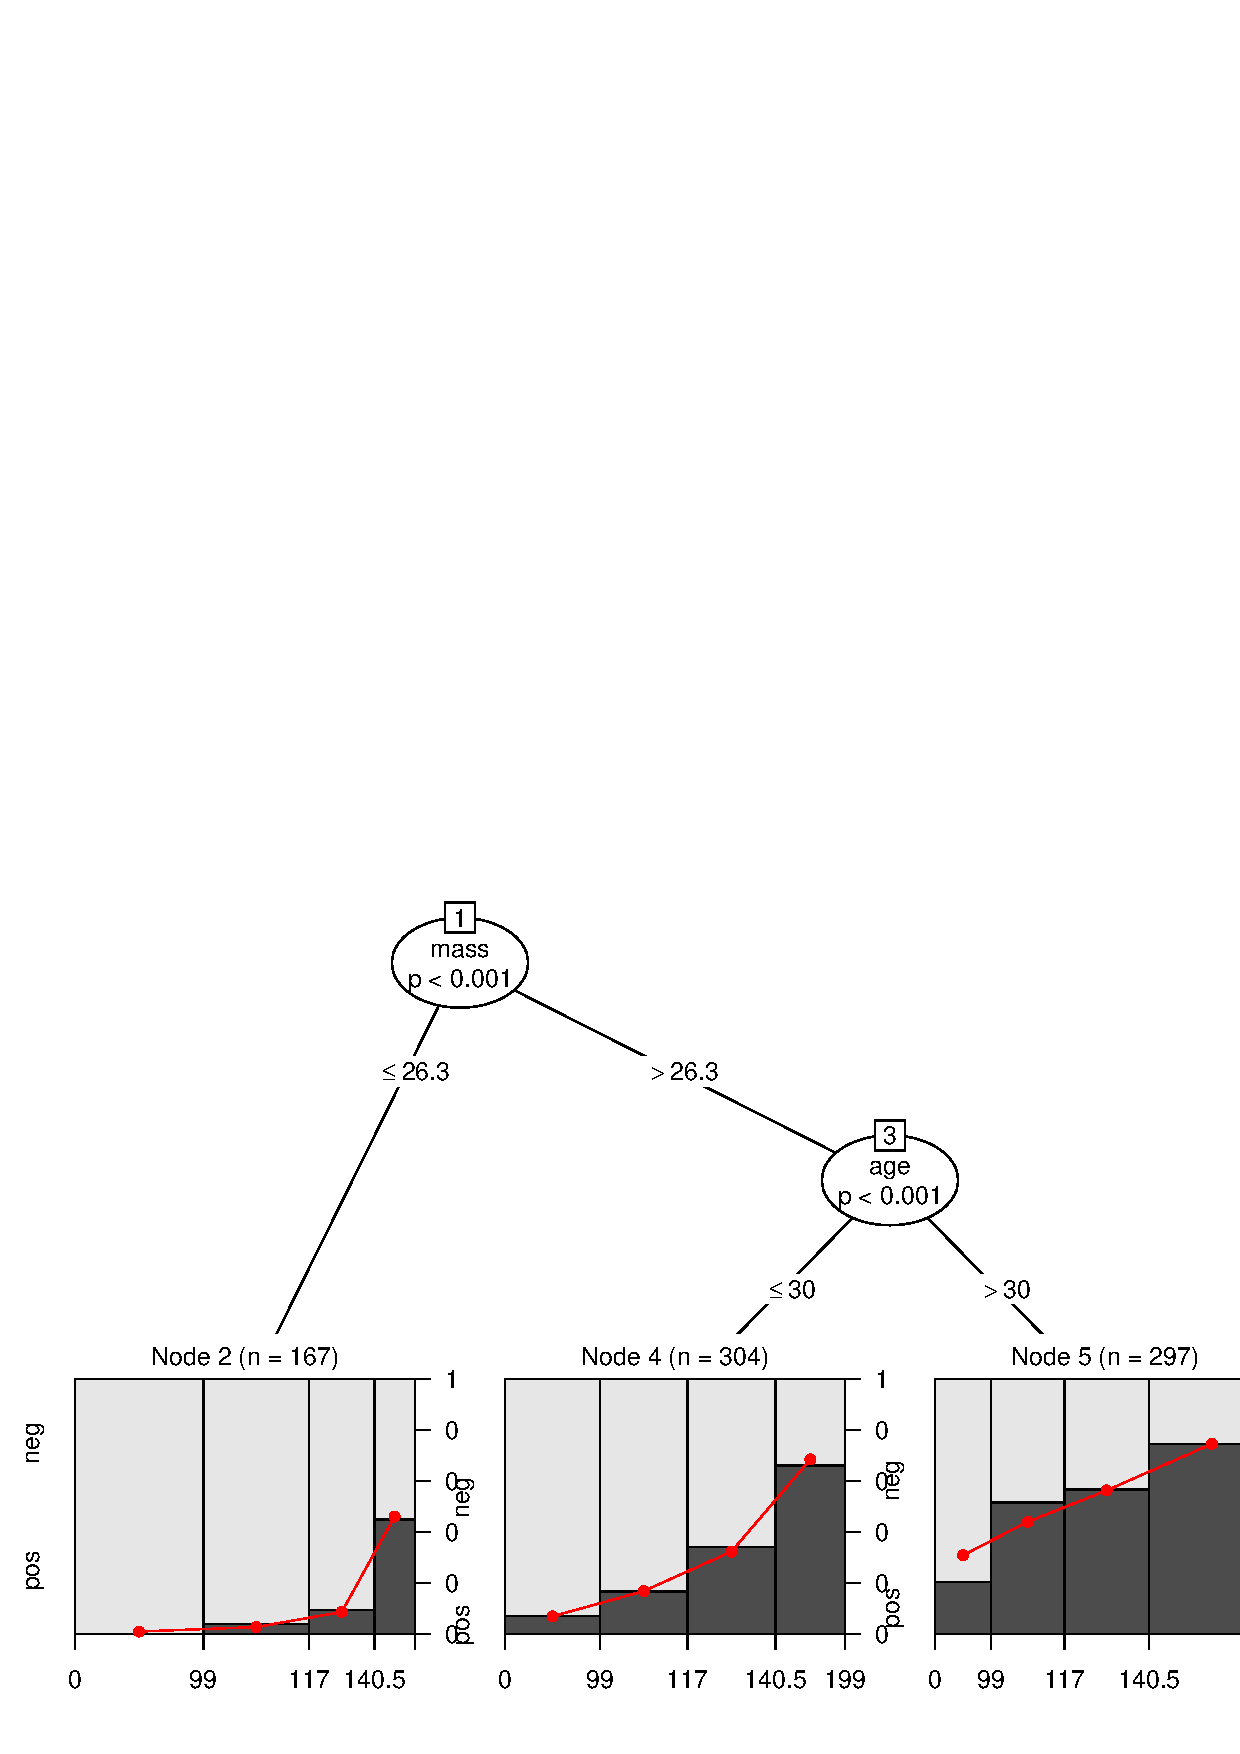
\includegraphics{MOB-PimaIndiansDiabetes-plot}
\caption{\label{fig:PimaIndiansDiabetes} Logistic-regression-based tree for the Pima Indians
diabetes data. The plots in the leaves give spinograms for \code{diabetes} versus 
\code{glucose}.}
\end{center}
\end{figure}

which produces again a plot of the dependent variable $y$ against the only regressors
$x$ in the terminal nodes. As $y$ is \code{diabetes}, a binary variable, and $x$ is 
\code{glucose}, a numeric variable, a spinogram is chosen for visualization. The breaks
in the spinogram are the five-point summary of \code{glucose} on the full data set. The
fitted lines are the mean predicted probabilities in each group.

The model tree distinguishes three different groups:
\begin{itemize}
  \item[\#2] Women with low body mass index that have on average a low risk of
    diabetes, however this increases clearly with glucose level.
  \item[\#4] Women with average and high body mass index, younger than 30 years,
    that have a higher avarage risk that also increases with glucose level.
  \item[\#5] Women with average and high body mass index, older than 30 years,
    that have a high avarage risk that increases only slowly with glucose level.
\end{itemize}

The same interpretation can also be drawn from the coefficient estimates
and the corresponding odds ratios (with respect to glucose):

\begin{Schunk}
\begin{Sinput}
> coef(fmPID)
\end{Sinput}
\begin{Soutput}
  (Intercept)    glucose
2   -9.951510 0.05870786
4   -6.705586 0.04683748
5   -2.770954 0.02353582
\end{Soutput}
\begin{Sinput}
> exp(coef(fmPID)[,2])
\end{Sinput}
\begin{Soutput}
       2        4        5 
1.060465 1.047952 1.023815 
\end{Soutput}
\end{Schunk}


i.e., the odds increase by 6\%, 4.8\% and 2.4\%
with respect to glucose in the three groups.



\section{Conclusion}
\label{sec:conclusion}

The function \code{mob()} in the \pkg{party} package provides a flexible and object-oriented
implementation of the general algorithm for model-based recursive partitioning.
Models of class ``\code{StatModel}''---that employ a formula interface and are equipped with
methods for the generic functions \code{reweight()}, \code{weights()}, \code{estfun()} plus
some function for extracting the value of the objective function---can be easily partitioned.
The resulting ``\code{mob}'' tree can be flexibly summarized, both numerically and graphically,
and used for predictions on new data.


\bibliography{partyrefs}

\end{document}
